%\documentclass[convert={convertexe={magick.exe},density=900,size=900x600,outext=.png,class=article}]{standalone}
\documentclass[12pt]{article}
\usepackage[left=2cm,right=2cm,top=1.5cm, bottom=1.5cm,paperheight=27.5cm]{geometry}
\usepackage{enumitem}
\usepackage{graphicx}
\usepackage{tikz}
\usepackage{etoolbox}
\usepackage{multicol}

\newcommand{\circleChar}[3][]{%
	\node[shape = circle, draw, inner sep = 1pt, fill = red!80!black] at (#3)
    (char) {\phantom{\ifblank{#1}{#2}{#1}}};%
    \node[text = white] at (#3) {\makebox[0pt][c]{#2}};}
\newcommand{\circled}[2][]{%
  \tikz[baseline=(char.base)]{%
  		\circleChar[#1]{#2}{char.center}}}
\robustify{\circled}
\newcommand{\dcircled}[1]{\circled[00]{#1}}

\newcommand{\rectangled}[2][]{%
  \tikz[baseline=(string.base)]{%
    \node[shape = rectangle, line width=1mm, draw, inner sep = 5pt, #1, text = black] (string) {#2};}}
\robustify{\rectangled}

\pagestyle{empty}

\begin{document}

%\begin{center}
%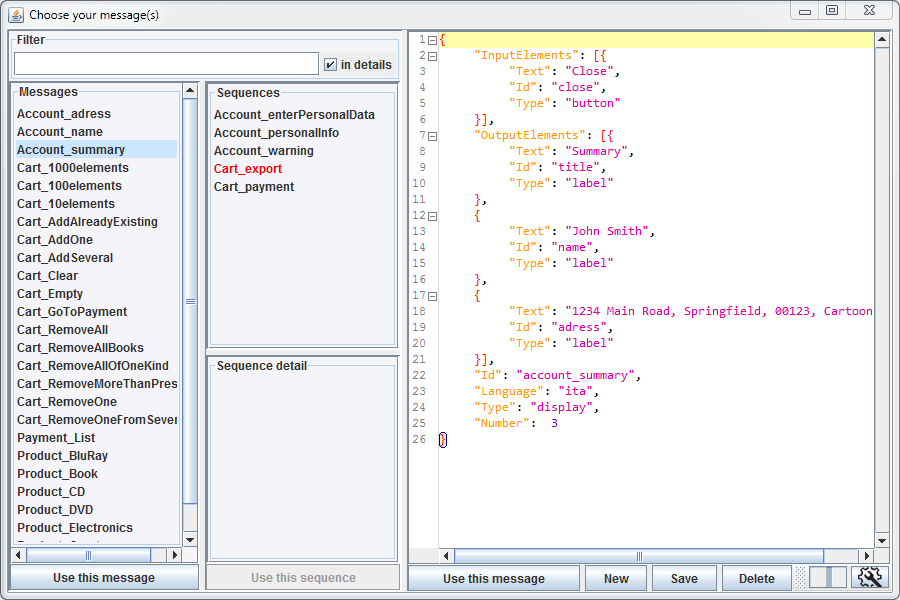
\includegraphics[width=\textwidth]{../Screenshots/00_MessagePicker.png}
%\end{center}
\begin{center}
\begin{tikzpicture}
    \node[anchor=south west,inner sep=0] (image) at (0,0) {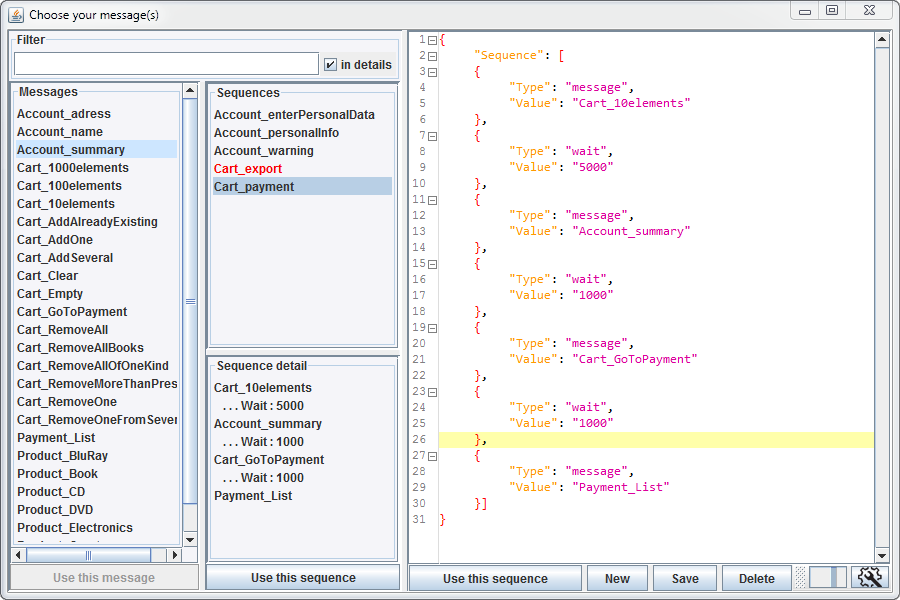
\includegraphics[width=\textwidth]{../Screenshots/01_MainWindow.png}};
    \begin{scope}[x={(image.south east)},y={(image.north west)}]
    
%\draw[help lines,xstep=.1,ystep=.1] (0,0) grid (1,1);   
    
    	\draw[green,line width=1mm] (0.01,0.01) rectangle (0.22,0.872);
    	\draw[yellow,line width=1mm] (0.228,0.01) rectangle (0.442,0.872);
    	\draw[blue,line width=1mm] (0.65,0.01) rectangle (0.885,0.06);
    	\draw[violet,line width=1mm] (0.45,0.07) rectangle (0.985,0.95);
    	
		\circleChar[00]{1}{0.975,0}
		\circleChar[00]{2}{0.92,0}
		\circleChar[00]{3}{0.2,0.026}
		\circleChar[00]{4}{0.42,0.026}
		\circleChar[00]{5}{0.625,0.026}
		\circleChar[00]{6}{0,0.74}
		\circleChar[00]{7}{0.42,0.68}
		\circleChar[00]{8}{0.08,0.925}
    	
    \end{scope}
\end{tikzpicture}
\end{center}

\vspace{.8cm}

\begin{tabular}{l@{\hspace{1em}}l}
\rectangled[green]{Pick a message} 	& List of all saved messages.\\
\rectangled[yellow]{Pick a sequence} & List of all saved sequences. \\
									& When a sequence is selected, its steps are listed below. \\ 
\rectangled[blue]{Manage actions} 	& Create an action, save it or delete it. \\ 
\rectangled[violet]{Edit action} 	& A Json editor to edit messages and sequences. \\ 
\end{tabular}

\vspace{.8cm}

\begin{multicols}{2}
\begin{enumerate}[label=\dcircled{\arabic*}]
	\item Open/Close configuration file editor
	\item If \emph{'loading'}, means the server is running and the renderer can receive the picked action.
	\item Pick a message to be sent to the renderer. Only active if a message is selected.
	\item Pick a sequence to be sent to the renderer. Only active if a sequence is selected.
	\item Pick the action shown in the editor to be sent to the renderer.
	\item Current action: picked action currently sent to the renderer.
	\item Selected action: action currently shown in the editor.
	\item Filter all action lists (case insensitive).
\end{enumerate}
\end{multicols}

\end{document}


% Image magick commands to transform in png or jpg:
%
%%%% Jpeg
%
% 	magick -density 300 -quality 90 MessagePicker.pdf MessagePicker.jpg
%
%%%% Transparent png
%
%	magick -density 300 -quality 90 MessagePicker.pdf MessagePicker.png
%
%%%% Non-transparent png
%
%	magick -density 300 -quality 90 MessagePicker.pdf -background white -alpha remove  MessagePicker.png